\documentclass{standalone}
\usepackage[svgnames]{xcolor}
\usepackage{tikz}
\usepackage{times}

\begin{document}

% T10I4D100K 1\%
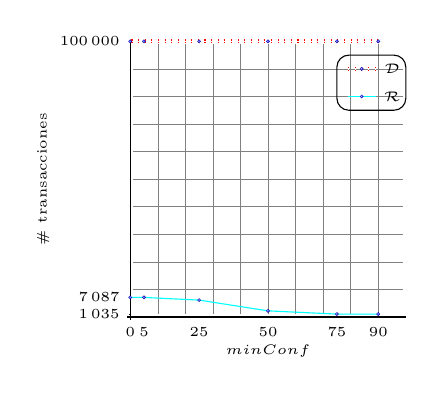
\begin{tikzpicture}[scale=.35]
   %ejes
   \draw (-0.1,0) -- (10,0);
   \draw (0,-0.1) -- (0,10);
   \draw[help lines,step=1cm] (0.1,0.1) grid (9.9,9.9);
   %marcas
   %       \foreach \x in {0,0.1,0.5,2.5}
   %           \draw (\x cm,1pt) -- (\x cm,-1pt) node[anchor=north] {\tiny $\x$};
   %marcas eje X
   \draw (5cm,-35pt) node {\tiny $minConf$};
   \draw (0cm,1pt) -- (0cm,-1pt) node[anchor=north] {\tiny 0};
   \draw (.5cm,1pt) -- (.5cm,-1pt) node[anchor=north] {\tiny 5};
   \draw (2.5cm,1pt) -- (2.5cm,-1pt) node[anchor=north] {\tiny 25};
   \draw (5cm,1pt) -- (5cm,-1pt) node[anchor=north] {\tiny 50};
   \draw (7.5cm,1pt) -- (7.5cm,-1pt) node[anchor=north] {\tiny 75};
   \draw (9cm,1pt) -- (9cm,-1pt) node[anchor=north] {\tiny 90};
   %marcas eje Y
   \draw (-90pt,5 cm) node[rotate=90] {\tiny \# transacciones};
   \draw (1pt,.1035 cm) -- (-1pt,.1035 cm) node[anchor=east] {\tiny 1\,035};
   \draw (1pt,.7087 cm) -- (-1pt,.7087 cm) node[anchor=east] {\tiny 7\,087};
   \draw (1pt,10.0000 cm) -- (-1pt,10.0000 cm) node[anchor=east] {\tiny 100\,000};
   %       \draw (-0.2,-0.5) -- node[right=1pt,fill=white] {\tiny 5\%};
   %líneas
   \draw[color=red,style=dotted,double] plot[mark=ball] coordinates {
      (9.0, 10.0000)
      (7.5, 10.0000)
      (5.0, 10.0000)
      (2.5, 10.0000)
      ( .5, 10.0000)
      % ( .1, 10.0000)
      (  0, 10.0000)
   };
   \draw[color=Aqua,style=solid] plot[mark=ball] coordinates {
      (9.0, .1035)
      (7.5, .1035)
      (5.0, .2211)
      (2.5, .6109)
      ( .5, .7087)
      % ( .1, .7087)
      (  0, .7087)
   };
   %leyenda
   \draw[rounded corners=1ex] (7.5,7.5) rectangle (10,9.5);
   \draw (9.5,9) node(a) {\tiny$\mathcal{D}$};
   \draw (9.5,8) node(a) {\tiny$\mathcal{R}$};
   \draw[color=red,style=dotted,double] (7.9,9) -- (8.9,9) plot[mark=ball] coordinates {(8.4,9)};
   \draw[color=Aqua,style=solid] (7.9,8) -- (8.9,8) plot[mark=ball] coordinates {(8.4,8)};
\end{tikzpicture}

\end{document}